\subsection{Using statistics to calculate uncertainty}

By now in a experimental design, I am usually at my tolerance limit for calculating uncertainties. You might ask, can't we get our powerful computers to help us out a little bit with finding the uncertainty? After all, we went to all the trouble to get the data on the computer. The answer is, yes!

Let's suppose we have done our experiment and we have some data that look like this: 

\begin{figure}[h!]
	\centering
	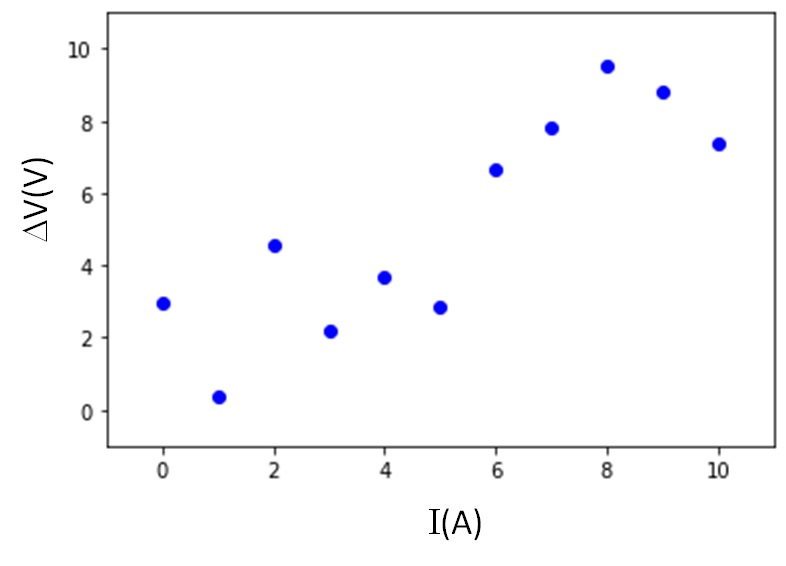
\includegraphics[width=3.563in,height=2.7345in]{linear_data}
\end{figure}

This looks pretty good. It seems to be sort of linear. We might guess from this that Ohm's law is begin obeyed. But we want $R_{test}$ and $R_{test}$ is the slope of this line. We could calculate $R_{test}$ from each pair of $\Delta V$ and $I$ points and find it's uncertainty using standard error propagation. But it seems that it would be better to take all the points into our analysis to find $R_{test}.$ More data should give us a better estimate for $R_{test}.$ Back in PH150 you may have done such a thing using a \emph{curve fit}. In the next figure, a curve fit is shown for the data from the last figure. 

\begin{figure}[h!]
	\centering
	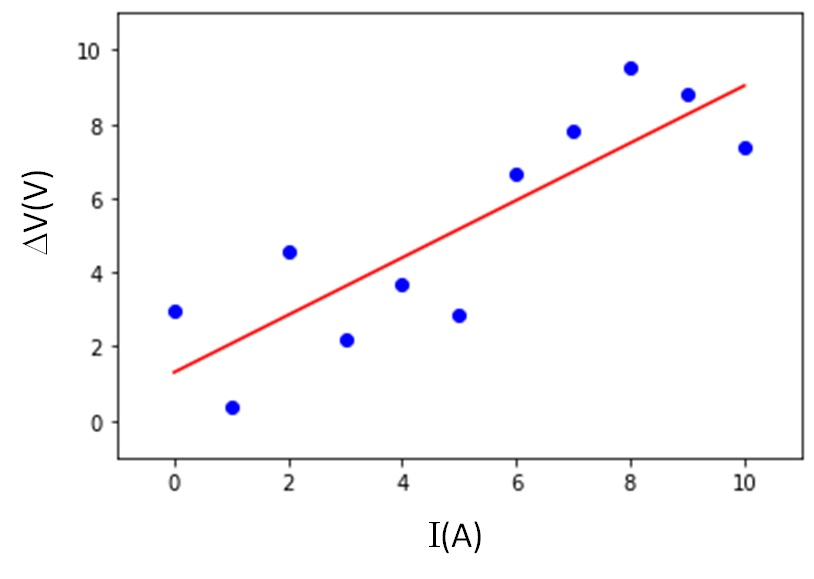
\includegraphics[width=3.563in,height=2.7345in]{linear_data_with_fit}
\end{figure}

Notice that I performed this curve fit in python, but if you are a not a great Python programer you could do this in Excel. You could also do this in LoggerPro or many other data analysis programs. If you need help finding a way to perform a curve fit, talk to your instructor. Here is an example code for doing the curve fit in python.

\vspace{0.24in}
\href{https://raw.githubusercontent.com/rtlines/IntermediateLabPH250/main/Code/linear_fit.py}{Download here}

\lstinputlisting[language=Arduino]{Code/linear_fit.py}

The scipy linregress() function uses the equation for a line 

\begin{equation*}
	y = result.slope*x + result.intercept
\end{equation*}

\noindent Our code gives the result

\begin {verbatim}
slope is   0.7737292152727273 +-  0.1612215125332822
intercept is   1.2996514309090914 +-  0.9537993308988922
program ended successfully
\end{verbatim}

\noindent which tells us that we have a slope of about $0.774.$ Since our graph
has $\Delta V$ on the vertical axis and $I$ on the horizontal axis we
recognize 
\begin{eqnarray*}
	\Delta V &=&R_{test}I+0 \\
           y &=&mx+b
\end{eqnarray*}

that $R_{test}$ must be the slope. We can see that the resistance is about a tiny $0.774\unit{\Omega}$ because that is the slope of our fit line. But we know we need an uncertainty along with this nominal value. And low and behold! the scipy lineregress() function has already given us the data we need to find the errors on the slope and intercept as well! This was pretty easy!

Notice that in this analysis technique, we can often afford some error in our 
$\Delta V$ and $I$ values. So maybe a $9\%$ error (like we found in one of
our instrument designs) is not so bad. We may not have to work too hard to
get a wonderful choice of shunt resistor if we are going to use many data
points and the power of statistics to analyze the data in the end!
